\chapter{Monte Carlo Tree Search}
\label{ch_mcts}

Monte Carlo methods\footnote{Not to be confused with
Monte Carlo algorithms which are precisely defined as the algorithms
solving the decision problems in classes BPP and RP.} are using random sampling to estimate the correct
solution to a problem. The first serious use of Monte Carlo methods was
by Stanislaw Ulam and John von Neumann during their work on the
Manhattan project, but the technique has since spread into many areas of
science due to its general applicability.

One of the celebrated Monte Carlo methods
is the simulated annealing algorithm (so called due to its
origin in statistical physics) which is an improved version of
Metropolis algorithm (invented by a Manhattan project scientist
Nicholas C. Metropolis and others).

This method found its way into game
theory in 1993 when it was applied to the board game Go
\parencite{MonteCarloGo}. The approach was later further improved
\parencite{MonteCarloGoDevel} but the real breakthrough came in 2006
when Coulom \parencite{Coulom} and Kocsis, Szepesvári \parencite{Kocsis}
independetly explored the idea of maintaing a tree which would guide the
search for strategies -- thus discovering Monte Carlo Tree Search.
This was eventually used in the AlphaGo program
\parencite{alphago}, the first
computer program to beat professional human players.

Monte Carlo Tree Search (MCTS) is, in short, a
heuristic search algorithm for finding good strategies in complex
decision processes by combining standard approaches of artificial
intelligence and computational statistics: tree search and sampling.

In this chapter the general MCTS scheme is defined and a concrete instance
called UCT is shown together with its application to maximizing rewards
in MDPs and games. The chapter is based mostly on a thorough MCTS survey
paper \parencite{mcts_survey}.

Since the research into MCTS focuses mainly on using MCTS for reward maximization
we also focus on that in this chapter unlike the rest of the thesis.

TODO: define MDP with rewards here (but mention it in the mdp chapter
too, just briefly, informaly)

\section{General MCTS Scheme}

MCTS iteratively builds a tree which approximates possible resulting
rewards of strategies in the decision process. In each iteration the
tree guides the search to balance between exploitation of known good
strategies and exploration of new strategies. When the search leaves the
tree it proceeds at random and upon terminating it adds a new leaf to
the tree and updates its ancestors with the result. This is summarized
in \autoref{mcts}.


\begin{algorithm}
\caption{General Monte Carlo Tree Search method}
\label{mcts}
\begin{algorithmic}
\Function{MCTS}{$s_0$}
    \State Let $v_0$ be the root of the MCTS tree, with $v_0.state = s_0$.
    \While{within computational budget}
        \State $v_l \gets \Call{TreePolicy}{v_0}$
        \State $\Delta \gets \Call{DefaultPolicy}{v_l}$
        \State $\Call{Backup}{v_l, \Delta}$
    \EndWhile
    \State \Return Action from $v_0$ to the best node (by some
    given metric).
\EndFunction
\end{algorithmic}
\end{algorithm}

\section{Upper Confidence Bound for Trees}

The most common implementation of the general scheme is {\em Upper
Confidence Bound for Trees} (UCT) which utilizes formula \ref{UCB}.
In this formula $\overline{X}_i$ represents the expected outcome
from node $i$, $n$ is the number of visits to all nodes, $n_i$ is the
number of visits to node $i$. $C$ is an arbitrary constant.

\begin{equation}
\label{UCB}
UCT_i = \overline{X}_i + C \sqrt{ \frac{2 \ln n}{n_i} }
\end{equation}

Selecting a tree node which maximizes this value makes the algorithm balance
between exploitation of known good strategies and exploration of new.
Constant $C$ instructs the algorithm how much weight to give to
exploration. TODO: Mention the result of Kocsis and Sepe... which proves
$1/\sqrt(2)$ to be optimal under some circumstances.

\autoref{uct} is implementation of the general \autoref{mcts}. As UCT is
the most common type of MCTS algorithm, the terms are often used
interchangeably in literature.

TODO: Define precisely the problem uct is solving (it should be
maximization of rewards in MDP).

\begin{algorithm}
    \caption{Upper Confidence Bound for Trees}
\label{uct}
\begin{algorithmic}
\Function{UCT}{$s_0$}
    \State TODO
    \State Let $v_0$ be the root of the MCTS tree, with $v_0.state = s_0$.
    \While{within computational budget}
        \State $v_l \gets \Call{TreePolicy}{v_0}$
        \State $\Delta \gets \Call{DefaultPolicy}{v_l}$
        \State $\Call{Backup}{v_l, \Delta}$
    \EndWhile
    \State \Return Action from $v_0$ to the best node (by some
    given metric).
\EndFunction
\end{algorithmic}
\end{algorithm}

\section{Solving Games}

In this section a brief introduction to game theory is given, starting
with definitions of games, strategies and solutions to games. We
proceed by presenting the standard {\em minimax} algorithm, then showing
how MCTS can be used to solve games and how it compares with minimax.
Lastly we show how MCTS is used to play the game of Go, which has been a
fruitful subject of research.
Observing where it performs good and where it does not provides insight
into MCTS and is a useful starting point for understanding the results
of evaluation in \autoref{ch_evaluation}.


Our definition of a game is that of a {\em perfect-information
extensive-form game}. The perfect-information in games corresponds to
full observability in MDP.  The reader can notice other similarities
with MDPs as well, for example games have states, final states, actions
and enabled actions, as well as rewards. On the other hand the
transition function is deterministic.

\begin{definition}
    A {\em game} is a tuple $G = (N, S, F, A, E, \Delta, \rho, u)$,
    where
    \begin{itemize}
        \item $N \subseteq \mathbb{N}$ is a finite set of players,
        \item $S$ is a set of states,
        \item $F \subseteq S$ is a set of final (terminal) states,
        \item $A$ is the set of actions,
        \item $E : S \to \mathcal{P}^+(A)$ is a function which tells the player
            which non-empty set of actions can be played in a given state,
        \item $\Delta : S \times A \to A$ is the transition function,
        \item $\rho : S \to N$ is a function which determines who plays in each state,
            and finally
        \item $u = (u_1,\ldots,u_n)$ is the tuple of
            utility (reward) functions where each $u_i, i \in N$ is a function
            $u_i : F \to \mathbb{R}$.
    \end{itemize}
\end{definition}

TODO: there may be some more conditions I didn't realize in the definitions, check
ia168

Game starts in a distinguished state $s_0$ and players take turns until
a terminal state (in $F$) reached. In a turn a player in state $s$ chooses
action $a$ from $E(s)$ and the action leads to state $\Delta(s,a)$.
If the state $\Delta(s,a)$ is terminal, then every player $i$ receives
the reward $u_i(\Delta(s,a))$.

A common choice of the utility function is $+1, 0, -1$ for victory, draw
and loss, respectively.

\begin{example}
\end{example}

\begin{definition}
    A {\em strategy} of player $i$ in a game $G$ is a function
    $\pi_i : S \to \distribution{A}$, such that for all $s \in S$ and $a
    \in A$ it holds that if $\pi_i(s)(a) > 0$ then $a \in E(s)$.

    A {\em strategy profile} is an $N$-tuple with a strategy for each player.
\end{definition}

We assume the players are rational and thus pick strategies which
optimize for their goals. A goal may be to maximize the player's reward,
another goal may be to get a higher score than the opponents.

\begin{example}
    \label{example_goals}
    In the game below let Alice be player 1 and Bob player 2.
    There is a single turn made by Alice in the black node.
If her goal is to beat Bob she will pick the left node.
If her goal is to maximize her profit she will choose the right one.

    \begin{center}
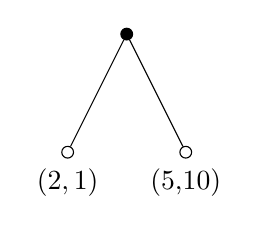
\begin{tikzpicture}
\tikzset{
solid node/.style={circle,draw,inner sep=1.5,fill=black},
hollow node/.style={circle,draw,inner sep=1.5}
}

\node(0)[solid node]{}
    child{node[hollow node,label=below:{$(2,1)$}]{}}
    child{node[hollow node,label=below:{(5,10)}]{}};
\end{tikzpicture}
\end{center}
\end{example}

For simplicity we restrict
ourselves to two player games in the following text unless otherwise
noted.


\subsection{Zero-sum games and minimax}

In zero-sum games one player wins at the cost of the other losing.
There are plenty of examples of such games, e.g. Chess, Go, which makes
them an important subject of study.

\begin{definition}
    Let $G = (N, S, F, A, E, \Delta, \rho, u)$ be a game.
    $G$ is said to be {\em zero-sum} if the rewards always sum to zero,
    that is $\sum_{i \in N} u_i(s) = 0$ for all $s \in F$.
\end{definition}

An important type of strategy is {\em minimax}. A player playing this
strategy is minimizing their potential maximum loss\footnote{Some might
prefer calling it {\em maximin} for maximization of the minimum reward,
which is equivalent to the first definition in zero-sum games.}. If both players play a
minimax strategy, the strategy profile is a Nash
equilibrium\footnote{
A strategic profile is a Nash equilibrium, if no player can get a higher
reward by switching a strategy.
    }$^,$\footnote{The {\em minimax theorem} was proven by John
von Neumann.}.

The {\em minimax algorithm} computes the value of each leaf in a game
tree assuming the opponent tries to harms the player as much as
possible. The algorithm then tells the player to play the action going
into the subtree with the highest value node.

\autoref{negamax}, the {\em negamax algorithm}, is a minor simplification
of minimax, equivalent to minimax in zero-sum games.

\begin{algorithm}
\caption{Negamax}
\label{negamax}
\begin{algorithmic}
\Function{negamax}{$node$}
    \If{$node$ is a leaf}
        \State \Return hmm.. how to write it
    \EndIf
    \State \Return $\max \{ - \Call{negamax}{child}
        \mid child \text{ of } node \}$
\EndFunction
\end{algorithmic}
\end{algorithm}

TODO: example execution

For larger games a variation called {\em minimax search} is used, which
performs the computation only to a limited depth, and then uses
a heurisic to evaluate the last node it processes (unless it is a leaf).

\subsection{Solving with MCTS}

From the negamax algorithm in the previous section there is an easy step
to solving games with MCTS. \autoref{mcts_negamax} is an
implementation of the Backup function in UCT for finding a good
action a player should take in a zero-sum game.

\begin{algorithm}
\caption{Negamax MCTS Backup}
\label{mcts_negamax}
\begin{algorithmic}
\Function{backup}{$v, \Delta$}
    \While{$v$ is not $null$}
        \State $N(v) \gets N(v) + 1$
        \State $Q(v) \gets Q(v) + \Delta$
        \State $\Delta \gets - \Delta$
        \State $v \gets $ parent of $v$
    \EndWhile
\EndFunction
\end{algorithmic}
\end{algorithm}

TODO: Example execution?

An important theoretical result is
that MCTS converges to minimax \parencite{Kocsis},
so eventually, after a lot of MCTS iterations, there is a negligible
difference between the results of the two methods and they pick the same
next move. However in
applications we want to know when to use minimax (\autoref{negamax}) and
when to use UCT (\autoref{uct} with \autoref{mcts_negamax}) without
iterating UCT for a long time.

While UCT achieved success in many games \parencite{mcts_survey},
for example in chess it does not perform well. The reason being that chess
games contain a lot of trap states (states from which the opponent
has a guaranteed victory) which are reachable just in a few turns. UCT
then spends a lot of time exploring these fruitless parts of the search
tree \parencite{mcts_vs_chess}.

\subsection{Computer Go}

Go is an example of a game where MCTS has proven to be a good choice,
most recently with the AlphaGo program \parencite{alphago}.
We shortly introduce Go and how MCTS is used to
play it.

The basic rules of Go are simple. The
standard board is a $9\times9$ (for beginners) or $19 \times 19$ grid.
Two players, black and white, alternate in their moves, each
placing a single stone of their color on an intersection of lines.
By surrounding the stones of the opponent a player captures all the
surrounded stones. The game ends when both players agree to end and the
winner is the player with greater sum of controlled territory and
captured stones.
The rules are well explained in detail at
\href{http://playgo.to/iwtg/en/}{http://playgo.to/iwtg/en/}.


TODO: How is MCTS used in some simple Go program.
Link to AlphaGo for advanced technique.

A Go player can observe that unlike in Chess there is seldom a quick way
to lose, as a loss of a small part of territory may be reversed, however
losing an important piece is hardly reversible. It seems plausible this
generalizes to territory versus piece based games.

We end our detour to games with Arimaa, a game specifically designed in
2002 to be easy for humans but hard for computers, for example by
allowing more moves per turn. Eventually Arimaa players lost to a
program in 2015 \parencite{arimaa}. The program uses techniques similar
to chess programs like alpha-beta pruning and on top of that employs
heuristics inspired by the best human players. See \parencite{jakl} for
MCTS related insights into Arimaa.
